\section{Background}

Signal processing community has successfully developed various
algorithms to capture and extract useful information from real world signals. As a result, the digital signal processing (DSP) have been widely deployed in many computational applications in areas such as image processing, video conferencing, smart sensors network, and other real-time processing applications that involve data acquisition.

However, with the amount of data collected
by such systems significantly increased in recent years, mainly due to the extremely high frequency and wider bandwidth communication systems, the challenges in acquiring signals at ever higher sampling rates becomes a serious and crucial problem in the front-end sampling circuits.

The Shannon/Nyquist sampling theorem \cite{wyner1998introduction} states that an original signal can recover without lost of information if the sampling can be done at least two times faster than the signals
bandwidth. As a result, in many DSP related
applications, e.g. digital image processing and video streaming, the Nyquist rate is so high that the amount of  samples generated are enormous , making compression a necessary prerequisite to storage or transmission.
In other words, the Shannon/Nyquist sampling requirments not only presents the most crucial limitations in fast sampling systems, it also produces large amount of data which leads to problems in efficient storing and transmission, that further lead to power management related issues.

\subsection{Compressed Sensing}

In recent years, a novel paradigm for signal processing and acquisition, the compressive sensing or compressed sensing (CS) technique, has been shown to have great potential to address the aforementioned sampling problems, and has also been demonstrated to be suitable for numerous computer and electronic engineering based applications. The CS utilises the notion that when the signals of interest contain only a relatively small number of significant components (we call it sparsity), known as sparse signal, sampling at the Nyquist rate is not necessary as well as inefficient. 

\todo[inline, color=green!40]{[CH:Mar08]The following words are newly added for a more clear statement for CS}
%ch
If we assume the original signal as $1 \times N$ vector, the observation behaviour can be modelled as a sensing matrix $A$ with a size of $m \times N$, and $m < N$. Then the sampling system can be described as
\begin{equation}\label{CS-model}
y = Ax
\end{equation}

Normally we cannot uniquely reconstruct the original signal $x$ because the system defined by (\ref{CS-model}) is underdetermined. But using the sparse information, the CS theorem \cite{candes2006robust} states that it is possible to uniquely reconstruct the signal using $O(k log (N/k))$ samples, where $k$ is the sparsity. This result so attractive in signal acquisition because the magnitude of required samples can be significantly decreased, so that the aforementioned sampling problem in Shannon/Nyquist sampling theorem can be solved by CS under the assumption of signal's sparsity.

Naturally, there are many signals directly have sparse information that suitable for the CS based sampling and reconstruction, such as images with low-rank matrix representation, and wireless channels with sparse impulse response coefficients. For those signals who has not apparent sparse structures, it is also possible to derive their approximate sparsity by using orthogonal basis representation or dictionary learning algorithms. As a result, most of physical signals can approximately presents their sparsity in the basis spanned domain and suitable for the CS applications\cite{candes2006robust, candes2006near, rudelson2008sparse, rauhut2012restricted}.

\section{Motivation and Objectives}

\todo[inline, color=green!40]{[CH:Mar08]I put the topic CSP in the latter section of cognitive radio. Now in this section, I only talk about general motivations for CS based signal processing, especially for wideband wireless signals. The sentences are all revised based on your last feedback}

The main focus of the research work is to further extend the CS based signal acquisition techniques for CS based data processing, particular in the wireless based applications. Using this approach, the proposed directions of the research will encompass various areas such as data compression, data acquisition, data storage, data transmission, optimal recovery and processing. Specifically, the focus will be for wideband signal processing based application since the requirement of sampling wideband spectrum are much more demanding than narrow band signals. The following subsections present the related objectives for the focus.

\subsection{Wideband Analog-to-Digital Converters}

Modern digital signal processing applications deal with a large amount of data, resulting in enormous numbers of observations and requiring high speed sampling in the front-end analog-to-digital converters (ADCs) of systems according to the Shannon/Nyquist sampling theorem. However, non-ideality error, design complexity, and energy cost are proportional to the high sampling rate and seriously affect systems' performance. 

Since the CS has the potential to reduce the required number of observations, then it is possible to reduce the sampling rate of the ADCs, then the problem caused by high sampling rate can be overcome along with the serious effects in system performance.

\subsection{Ultra Wideband Communication Systems}

\todo[inline, color=green!40]{[CH:Mar08]As your comment, I omit some details for UWB-transmitters and our energy aware design.}

Ultra wideband (UWB) based wireless communication is associated with features such as extreme wide transmission bandwidth, low-power consumption and shared spectrum resources \cite{paredes2007ultra}.
However, sampling of such high frequency (in ranges of GHz) or wideband signals is a challenging problem.

\begin{figure}[tbh]
\begin{center}
\noindent
  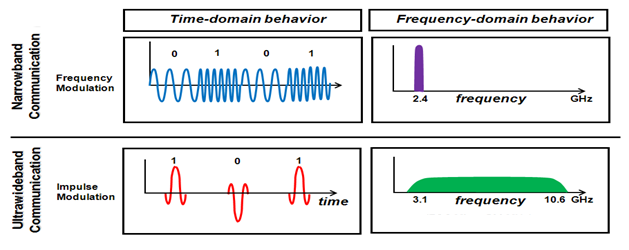
\includegraphics[width=0.7\textwidth]{UWB_signals.png}
  \end{center}
    \caption{Comparison of UWB signals vs narrow band signals in time and frequency domain.}\label{UWB_signals}
\end{figure}

The UWB signal displays sparsity when viewed in time domain (Figure \ref{UWB_signals}).  
Therefore, it is possible to embed the CS into UWB systems to reduce the required sampling rate: the CS sensing matrix can be a combination of the multipath channel with pre-mixing waveform done at receivers; the original signal is the UWB signal with time domain sparsity.

To implement the CS on UWB, there is no need to add any complex hardware for down-conversion such as matched filters or oscillators. All needed is a random mixing procedure before ADC's input, and then the low rate  sampling can be achieved based on the CS theory. As a result, compressed sensing would be appropriate to reduce the sampling rate while keeping flexibility for UWB systems. 

%\subsubsection{Energy Aware Design}

\subsection{Cognitive Radio}

Cognitive Radio (CR) is used to address the limited spectrum resource that seriously restricts the rapidly increasing demand for more accessible bandwidth.  However, studies \cite{larsson2008cognitive} indicate that many spectrum resources are actually unused in terms of time and space domain. This is termed as the spectrum holes, which are displayed the idle channel
in Figure \ref{CR_system}. The idea of exploiting such spectrum holes dynamically has led to the concept of cognitive radio \cite{axell2012spectrum}, where licensed spectrum dedicated to a primary network
would be reused by secondary (cognitive) devices dynamically when the primary user is idle.

\begin{figure}[tbh]
\begin{center}
\noindent
  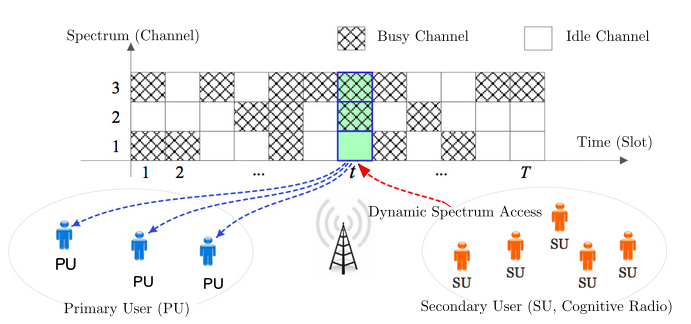
\includegraphics[width=0.7\textwidth]{CR_system.png}
  \end{center}
    \caption{Example of spectrum reuse and dynamic spectrum access for cognitive radios.}\label{CR_system}
\end{figure}

The cognitive devices cannot generate any harmful interference to the primary systems, so they needs to be kept at a distance
from the primary system, or transmit at relatively low energy levels. However, the CR would need to be of sufficient wideband sensitivity to monitor the spectrum utilization situation. 

As illustrated in in Figure \ref{CR_system} each secondary users needs to be fully aware of when and which sub-bands are idle, such that dynamical spectrum access or hand-off can be performed efficiently. As a result, the cognitive radios have to detect the presence of weak and wideband primary signals at a low energy level, and this problem is proposed as an fundamental issue in spectrum sensing \cite{sahai2004some}. 

Due to the low spectrum utilisation, the wideband spectrum is inherently sparse, which meets the requirements for the use of the  compressive sensing techniques. The CS spectrum sensing is hence a promising candidate to detect such wideband spectrum utilisation while using sub-Nyquist sampling rates \cite{sun2013wideband}.

\begin{figure}[tbh]
\begin{center}
\noindent
  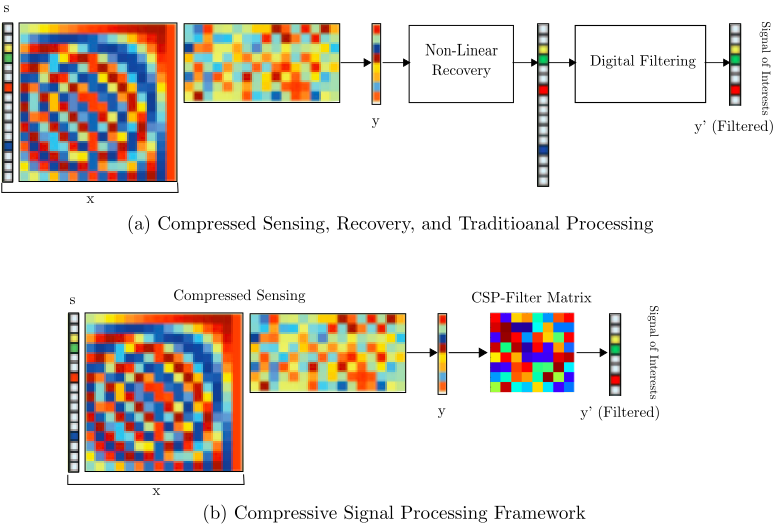
\includegraphics[width=0.7\textwidth]{CSP_system.png}
  \end{center}
    \caption{Filtering based scenario for comparison between (a) traditional digital signal processing via compressive measurements and (b) compressive signal processing (CSP)
framework.}\label{CSP_system}
\end{figure}

\subsubsection{Compressive Signal Processing}

\todo[inline, color=green!40]{[CH:Mar08]In this part, I begin to talk about the CSP, and briefly introduce our recommend CSP-CR devices model}

Most of tasks in cognitive spectrum sensing are related to detection, estimation, filtering, or classification rather than general CS task such as 'sample-then-recovery' procedures. As a result, a new research branch for the CS, the
compressive signal processing (CSP) \cite{davenport2010signal}, can be proposed to simplify the complexity of general CS work through directly
extracting useful information from the compressive samples without performing fully recovery, which is shown as Figure \ref{CSP_system}. 

Thus the CSP becomes a suitable candidate for CR that avoid the latency and inefficiency encountered in CS recovery process, while at the same time enable the usage of flexible and programmable digital system. 

\begin{figure}[tbh]
\begin{center}
\noindent
  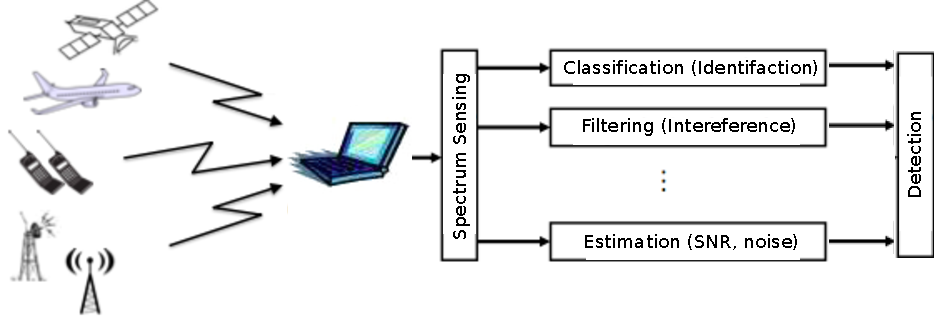
\includegraphics[width=0.7\textwidth]{CSP_CR_system.pdf}
  \end{center}
    \caption{The CSP based cognitive spectrum sensing for hybrid primary signals}\label{CSP_CR_system}
\end{figure}

For instance, the Figure \ref{CSP_CR_system} presents the CSP based cognitive spectrum sensing (CSS), which is able to detect and process various co-existed primary signals by using multiple hybrid processing methods such as classification or filtering. In this way, the CSP based CSS can provide better sensing adaptivity and flexibility for modern heterogeneous CR networks. 

\section{Organization of the Report}

The report is organized as follows:

\begin{enumerate}
\item Chapter \ref{CH1} introduces our main topic for CS based signal processing, including the background, motivation and objectives in this report.  
\item Chapter \ref{CH2} shows presents the background of
compressed sensing theory.
\item Chapter \ref{CH3} shows a survey done for recent CS-ADC architectures.
\item Chapter \ref{CH4} propose our related work in CS-UWB positioning systems.
\item Chapter \ref{CH5} demonstrates the CS spectrum sensing in cognitive radios.

\item Chapter \ref{CH6} draws a conclusion for the report and introduce our future research plans and areas that focus on compressive signal processing based cognitive spectrum sensing and access.
\end{enumerate}

